% BudgetBench expanded pilot paper.
% Compile from the paper/ directory with: tectonic main.tex

\documentclass[11pt]{article}

\IfFileExists{neurips_2026.sty}{\usepackage[eandd]{neurips_2026}}{}

\usepackage[utf8]{inputenc}
\usepackage[T1]{fontenc}
\usepackage[margin=1in]{geometry}
\usepackage{hyperref}
\usepackage{url}
\usepackage{booktabs}
\usepackage{amsfonts}
\usepackage{amsmath}
\usepackage{amssymb}
\usepackage{microtype}
\usepackage{graphicx}
\usepackage{xcolor}
\usepackage{multirow}
\usepackage{array}
\usepackage{longtable}
\usepackage{enumitem}
\usepackage[numbers]{natbib}
\emergencystretch=2em

\newcommand{\BudgetBench}{\textsc{BudgetBench}}
\newcommand{\RunModel}{\texttt{qwen2.5:1.5b}}
\newcommand{\RunId}{\texttt{final\_qwen25\_15b\_89items}}
\newcommand{\OllamaEndpoint}{\url{http://localhost:11434/v1/chat/completions}}

\title{\BudgetBench: A Budget-Tiered Benchmark for Memory Strategy Evaluation in Local LLM Agents}

\author{%
  Anonymous Author(s)\\
}
\date{}

\begin{document}

\maketitle

\begin{abstract}
Local large language model deployments are increasingly feasible, but active
context remains constrained by memory capacity, prefill latency, cache growth,
and application-level service objectives.  Memory-management strategies such
as truncation, summarization, retrieval, and hierarchical storage are therefore
not interchangeable implementation details; they determine which evidence is
available to the model under a fixed input budget.  We present \BudgetBench{},
an evaluation protocol and reference implementation for comparing memory
strategies across fixed active-context budget tiers.  The protocol holds the
model, task, sampler, and decoding parameters fixed; sweeps budgets over 2K,
4K, 8K, 16K, and 32K tokens; and records quality, budget utilization, latency,
and budget-violation rates.  We report a local pilot conducted on June 16,
2026 with Ollama and \RunModel{} over 89 SWE-bench Verified scaffold items
and 89 LongBench v2 items.  The pilot evaluates sliding-window truncation,
summary-buffer compression, and episodic retrieval at all five budget tiers.
We also include a three-item LongBench v2 transfer check for
\texttt{gemma4:e2b}.  Additional Qwen text and Qwen-VL tags were executed but
are excluded from the main tables because their text-only exact-match cells
were uninformative or dependent on serving configuration.  To evaluate the
multimodal serving path separately, we include a six-item synthetic image
question-answering probe for \texttt{qwen3-vl:2b}.  The results exhibit
non-monotonic quality curves, tight-budget compliance failures,
model-dependent behavior, limited multimodal endpoint viability, and
substantial latency differences across strategies.  We present these results
as pilot evidence, not as final strategy rankings, and provide the protocol,
implementation details, limitations, reproducibility checklist, and planned
extensions required for a larger community benchmark.
\end{abstract}

\section{Introduction}

Recent language models increasingly advertise context windows containing tens
or hundreds of thousands of tokens.  This trend can make explicit memory
management appear unnecessary: if the model can accept the entire trace, the
choice among retrieval, summarization, and truncation may seem secondary.
Local deployment conditions contradict this assumption.  A workstation,
laptop, or edge device may run an 8B or 14B model comfortably at short context
lengths but become slow or memory-constrained at longer lengths.  Even when a
long context fits in memory, an application may not tolerate the associated
prefill latency, memory pressure, or energy cost.  For local agents, active
context is an operational resource.

\BudgetBench{} is motivated by a practical question: \emph{given a fixed local
model, a fixed task, and a fixed active context budget, which memory strategy
should an agent use?}  The answer is not generally reducible to maximum context
length.  A truncation policy may be inexpensive but discard early evidence.  A
summary policy may preserve high-level state but introduce additional model
calls and summary drift.  Retrieval may preserve relevant evidence at tight
budgets but fail when the query is underspecified or when the retrieval corpus
is not chunked at a useful granularity.  Hierarchical memory systems such as
MemGPT-style stores and production systems such as Mem0 introduce additional
state and extraction policies, which may improve recall but also complicate
reproducibility \citep{packer2023memgpt,chhikara2025mem0}.

Existing benchmarks address related problems.  SWE-bench evaluates whether
models can produce patches for real GitHub issues \citep{jimenez2023swebench}.
LongBench and LongBench v2 evaluate long-context understanding across diverse
language tasks \citep{bai2023longbench,bai2024longbenchv2}.  RULER and HELMET
stress-test long-context behavior across synthetic and application-centric
length scales \citep{hsieh2024ruler,yen2024helmet}.  Lost-in-the-Middle shows
that accepting longer inputs does not imply reliable use of relevant
information throughout the sequence \citep{liu2023lost}.  Agent benchmarks such
as $\tau$-bench evaluate tool-mediated interaction in realistic domains
\citep{yao2024taubench}.  These benchmarks are valuable, but they do not
standardize the independent variable that local-agent developers routinely
control: the active context budget assigned to each model call.

This paper contributes a budget-tiered protocol and a pilot implementation.
The implementation is intentionally modest.  It includes a
\texttt{MemoryStrategy} interface, a budget-enforced evaluation harness, JSONL
metric logging, and reference implementations for truncation, summary-buffer
compression, and retrieval-augmented context selection.  The pilot run uses a
small local model and 89 items per task to obtain a denser pilot curve while
remaining reproducible on a single machine.  The resulting numbers should not
be read as final rankings.  They provide an empirical validation of the
measurement surface: \BudgetBench{} can expose quality curves, compliance
failures, and runtime tradeoffs that would be invisible in a single-budget
evaluation.

\paragraph{Contributions.}
This work makes six contributions.  First, it defines active-context-budget
evaluation as a protocol distinct from standard long-context model evaluation.
Second, it documents an implementation whose strategy interface admits new
memory policies without modifying task logic.  Third, it reports an 89-item
local pilot with complete five-tier tables for quality, violation rate, budget
usage, and duration.  Fourth, it adds a filtered small-model transfer check
showing how the same protocol can admit additional local text and
vision-capable model tags while excluding uninformative runs from result
tables.  Fifth, it adds a native image QA probe to separate multimodal serving
viability from text-only benchmark performance.  Sixth, it provides
reproducibility requirements and planned extensions for scaling
\BudgetBench{} from a local pilot to a public benchmark.

\section{Benchmark Definition}

\subsection{Objects and Notation}

Let $M$ denote a fixed local language model exposed through a chat-completion
API.  Let $T$ denote a task distribution with items $x \sim T$ and deterministic
grader $g(\hat{y}, x) \in [0,1]$.  Let $B$ be an active context budget measured
in tokens.  Let $\mathcal{S}$ be a set of memory strategies.  A strategy
$s \in \mathcal{S}$ maps an input message history $H = (m_1,\ldots,m_n)$ and
budget $B$ to a budget-constrained message list:
\[
  s(H, B) = H' \quad \text{such that} \quad \tau(H') \leq B,
\]
where $\tau$ is the benchmark tokenizer or tokenizer approximation.  The model
prediction is $\hat{y}=M(s(H,B))$, and the observed quality is $g(\hat{y},x)$.

The benchmark reports the empirical quality curve
\[
  Q(s, B, T, M) = \frac{1}{N}\sum_{i=1}^{N} g(M(s(H_i,B)), x_i),
\]
alongside utilization and reliability metrics.  The budget sweep is not a
model capability test in isolation; it is a controlled ablation over strategy
choice at fixed model, task, sampler, and decoding parameters.

\subsection{Active Budget Versus Nominal Context Window}

The active budget is the number of input tokens that the strategy is allowed
to present to the model for a particular call.  It is not the model's maximum
advertised context window, and it is not total task token cost.  This
distinction matters.  A model may support a 32K window while an application
allocates only 4K tokens to an interactive agent turn.  Conversely, an agent
may spend many total tokens across a task while each individual call remains
within a smaller active budget.  \BudgetBench{} isolates this per-call
constraint because that is the quantity memory strategies directly control.

\subsection{Rationale for Fixed Budgets}

Budget-tiered evaluation is useful for three reasons.  First, it creates
comparable operating points.  Reporting that a strategy performs well at
``short context'' is not precise; reporting quality at 2,048 tokens is.  Second,
it surfaces strategy crossovers.  Retrieval may dominate at 2K while
truncation may be sufficient at 16K.  Third, it reveals non-monotonic behavior.
Longer prompts can add distractors, shift relevant information away from
positions the model uses reliably, or trigger different generation behavior.
The long-context literature shows that larger context windows do not guarantee
reliable evidence use \citep{liu2023lost,hsieh2024ruler}; \BudgetBench{}
extends this observation to memory strategy comparisons.

\section{Related Work}

\subsection{Long-Context Benchmarks}

LongBench introduced a unified bilingual benchmark for long-context
understanding across single-document QA, multi-document QA, summarization,
few-shot learning, synthetic tasks, and code completion \citep{bai2023longbench}.
LongBench v2 shifts toward more demanding multiple-choice settings with long
contexts and reasoning-oriented questions \citep{bai2024longbenchv2}.  These
benchmarks are useful substrates for \BudgetBench{} because they expose
long-context evidence selection while retaining automatic grading.  However,
their default evaluation protocol asks how well a model handles a given long
input, not how well a memory strategy adapts the input to a fixed active
budget.

RULER evaluates long-context models with configurable synthetic tasks including
retrieval, multi-hop tracing, aggregation, and question answering
\citep{hsieh2024ruler}.  Its central lesson is that isolated retrieval success
can overstate long-context competence.  HELMET argues similarly for
application-centric evaluation across diverse long-context categories and
finds that synthetic tasks are not reliable predictors of downstream
performance \citep{yen2024helmet}.  \BudgetBench{} is complementary: it does
not replace long-context benchmarks, but instead imposes a fixed-budget axis
on task families where memory strategies are expected to matter.

\subsection{Agentic and Software Engineering Benchmarks}

SWE-bench grounds coding-agent evaluation in real repository issues and
patches \citep{jimenez2023swebench}.  SWE-bench Verified further filters the
benchmark to a human-validated subset of 500 instances.  In a full
\BudgetBench{} study, official containerized SWE-bench grading should be used.
The current pilot uses the public task data but replaces the official oracle
with deterministic patch-similarity scoring so that the budget matrix can be
run quickly on a single workstation.

$\tau$-bench evaluates tool-agent-user interaction in retail and airline
domains with domain APIs, policy documents, simulated users, and state-based
grading \citep{yao2024taubench}.  It is a strong candidate for future
\BudgetBench{} expansion because tool-use chains stress exactly the kind of
state retention, policy recall, and evidence selection that memory strategies
are designed to support.  The current repository contains a tau integration
path, but the pilot run omits it because the local tau2 data dependency was not
installed.

\subsection{Memory, Retrieval, and Compression}

Retrieval-augmented generation combines parametric model knowledge with
non-parametric retrieval, improving factuality and specificity on
knowledge-intensive tasks \citep{lewis2020rag}.  In the \BudgetBench{} setting,
retrieval is not merely a way to add external knowledge; it is a strategy for
selecting which internal task evidence enters a constrained prompt.  The RAG
baseline in this repository embeds intermediate messages, retrieves messages
relevant to the current query, and reconstructs a prompt that fits the active
budget.

MemGPT frames language-model memory as an operating-system-like hierarchy with
explicit management of context and archival stores \citep{packer2023memgpt}.
Mem0 presents a production-oriented memory layer that extracts, consolidates,
and retrieves salient conversational facts with substantial latency and token
savings relative to full-context approaches \citep{chhikara2025mem0}.  These
systems motivate richer strategy families than the three baselines used in the
pilot.  LLMLingua-2 represents a complementary compression family: rather than
choosing which chunks to include, it compresses prompt content toward a target
budget \citep{pan2024llmlingua2}.  \BudgetBench{} is designed to accommodate
these systems under the same interface once their dependencies and local
configuration are available.

\section{Evaluation Protocol}

\subsection{Budget Tiers}

The default budget tiers are 2K, 4K, 8K, 16K, and 32K tokens.  They are
log-spaced enough to reveal broad scaling trends while remaining recognizable
deployment regimes for local models.  A benchmark run should report every
strategy at every tier, even if some cells fail, because budget-compliance
failures are part of the measurement.  Missing cells make Pareto analysis
ambiguous; explicit failures preserve information about which strategies cannot
operate under a requested constraint.

\subsection{Strategy Contract}

The strategy contract is deliberately narrow.  A strategy receives a list of
chat messages and an integer budget.  It returns a list of chat messages.  The
runner then enforces the budget independently.  This separation prevents a
strategy from silently exceeding budget and avoids task-specific special cases.
Strategies may be stateful within a task item, but the runner resets them
between items in the current pilot.  Resetting makes the pilot easier to
interpret: each item is evaluated independently rather than benefiting from
cross-item memory.

\subsection{Task Contract}

A task provides three methods: dataset loading, task execution, and grading.
Execution is responsible for formatting a benchmark item as messages, invoking
the shared evaluation runner, extracting a prediction, and returning it to the
grader.  Grading must be deterministic.  This constraint is strict because
\BudgetBench{} is meant to compare small differences across budget tiers.  An
LLM-as-judge component could easily add variance larger than the effects under
study.

\subsection{Metric Contract}

Each cell logs raw per-item events and aggregate summary rows.  The primary
quality metric depends on the task: patch-similarity for the current SWE
scaffold and exact-match accuracy for LongBench v2.  The reliability metric is
budget violation rate.  The resource metrics are mean used budget, maximum peak
budget, duration, and tokens per task.  A full benchmark should also report
confidence intervals and repeated trials; the present pilot reports point
estimates because it is a bounded artifact-validation run.

\section{Implementation Details}

\subsection{Repository Structure}

The implementation is a compact Python package under \path{src/budgetbench}.
Core budget enforcement lives in \path{budgetbench/core}.  The evaluation runner
and metric logger live in \path{budgetbench/evaluation}.  Task adapters live in
\path{budgetbench/tasks}.  Strategy implementations live in
\path{budgetbench/strategies}.  The user-facing driver is
\path{scripts/run_pilot.py}; analysis and plotting utilities are in
\path{scripts/analyze_results.py} and \path{scripts/plot_tradeoffs.py}.

\subsection{Budget Enforcement Path}

For each item, the runner resets the strategy, applies it to the formatted
messages, counts tokens, and raises a budget exception if the processed prompt
exceeds the active tier.  The runner retries budget processing up to a fixed
limit.  If all retries fail, it logs a failed metric row with violation rate
1.0 for that item.  This design makes budget failures visible in the result
tables instead of hiding them as missing predictions.

\subsection{Logging and Analysis}

The raw logs are JSONL files, one per task-strategy-budget combination.  The
summary file records one aggregate row per cell.  The analysis script reads the
summary rows and then reopens per-cell logs to compute violation rate, mean
used budget, and maximum observed peak budget.  The analyzer supports both
older boolean \texttt{violation} fields and the current runner's numeric
\texttt{violation\_rate} rows.  This compatibility is important because a
table that reports all-zero violations while raw retry failures exist would
understate one of the key outcomes of budget-tiered evaluation.

\subsection{Multimodal Boundary}

The current benchmark task adapters are text-first: LongBench v2, the SWE
scaffold, and the tau integration path all produce chat messages.
This matters for interpreting vision-capable local model tags.  A
vision-language model can be served through the same local stack, but a
text-only LongBench prompt is not a multimodal benchmark.  In this revision,
the Qwen-VL text-only LongBench cells are treated as an excluded endpoint
check, while a separate six-item generated image QA set verifies the native
image-plus-text path.  A multimodal \BudgetBench{} extension should add
image or document-page payloads, visual question answering, chart/table
grounding, and multimodal retrieval policies under the same active-budget
discipline.

\section{Experimental Setup}

\subsection{Hardware and Serving}

The pilot was run locally on June 16, 2026 through Ollama's OpenAI-compatible
endpoint at \OllamaEndpoint.  The model was \RunModel{}, selected because it
could complete the full matrix within a practical runtime for local
experimentation.  The system also had larger MLX-backed models installed, but
those models produced reasoning-first responses through the local endpoint in
preliminary checks, which made them poorly suited for the exact-match pilot.
The \RunModel{} tag was installed locally through Ollama for the 89-item run.

After the primary 89-item run, we pulled additional local Ollama tags:
\texttt{gemma4:e2b}, \texttt{qwen3.5:0.8b}, \texttt{qwen3.5:2b}, and
\texttt{qwen3-vl:2b}.  All four tags responded through the OpenAI-compatible
chat path in preliminary checks.  We then ran a compact three-item LongBench v2
transfer check over the 2K, 4K, and 8K tiers using truncation and RAG.  The
paper reports only the informative \texttt{gemma4:e2b} rows.  The Qwen text
tags and the Qwen-VL tag are preserved in raw logs and in the consolidated CSV,
but excluded from the paper tables because their compact text-only exact-match
results were uniformly zero or required endpoint-specific generation settings
to avoid empty content.  We separately generated six simple colored-shape PNGs
and queried \texttt{qwen3-vl:2b} through Ollama's native image chat API; that
native multimodal probe is reported because it produced nonzero results.

\subsection{Sampling and Decoding}

The run uses 89 items per task.  For exact-match tasks, 89 examples produce
accuracy increments of approximately 0.0112, reducing the coarse quantization
of smaller pilot samples.  The decoding temperature is 0.0, the maximum
generation length is 512 tokens, and the random seed is 42.  The evaluated
matrix contains two tasks, three strategies, and five budget tiers, yielding
30 task-strategy-budget cells.

\subsection{Tasks and Graders}

The SWE task uses items from SWE-bench Verified and asks the model to output a
unified diff.  The pilot grader computes a patch-similarity proxy:
40\% file-level recall plus 60\% changed-line overlap on matched files.  This
metric is deterministic and cheap, but it is not equivalent to official
SWE-bench resolved rate.

The LongBench v2 task formats the context, question, and four choices as chat
messages.  The context is chunked into retrievable message parts before memory
strategy processing.  The grader extracts an answer letter and performs
exact-match scoring.  This task provides the more direct pilot measurement because
it is deterministic and natively multiple-choice.

\subsection{Baselines}

The pilot evaluates three baselines.  Truncation keeps the system prompt and
the newest messages that fit.  Summary-buffer compression summarizes evicted
context with the same local model and prepends that summary to the retained
messages.  RAG embeds intermediate context messages with a sentence-transformer
model, stores them in an in-memory Chroma collection, retrieves messages
relevant to the query, and reconstructs a prompt within the active budget.

\section{Results}

This section reports the 89-item run.  The complete raw logs are in
\path{logs/full_study/final_qwen25_15b_89items}.  The aggregate CSV and figures
are generated by the scripts in \path{scripts/}.  Table values are rounded to
two decimals in the main text and reported with additional operational metrics
in the appendix.
The main table separates LongBench v2 exact-match accuracy from the SWE
scaffold diagnostic.  The SWE cells are not official SWE-bench accuracy, and
the repeated high-budget proxy values occur because the selected SWE prompts
collapse into the same effective prompt regimes at the measured budgets rather
than because the strategies have independently identical coding performance.

\begin{table}[t]
\centering
\caption{Eighty-nine-item-per-task LongBench v2 pilot results for \RunModel. Quality is exact-match accuracy, and retrieval-augmented generation (RAG) denotes the episodic retrieval baseline.}
\label{tab:main_89item_results}
\resizebox{\textwidth}{!}{%
\begin{tabular}{lccccc|ccccc}
\toprule
& \multicolumn{5}{c|}{Quality} & \multicolumn{5}{c}{Violation rate} \\
Strategy & 2K & 4K & 8K & 16K & 32K & 2K & 4K & 8K & 16K & 32K \\
\midrule
Truncation & 0.29 & 0.27 & 0.27 & 0.33 & 0.33 & 0.00 & 0.00 & 0.00 & 0.00 & 0.00 \\
Summary & 0.30 & 0.24 & 0.26 & 0.29 & 0.31 & 0.03 & 0.07 & 0.05 & 0.07 & 0.03 \\
RAG & 0.30 & 0.31 & 0.35 & 0.34 & 0.31 & 0.00 & 0.00 & 0.00 & 0.00 & 0.00 \\
\bottomrule
\end{tabular}%
}
\end{table}

\begin{table}[t]
\centering
\caption{SWE-bench Verified scaffold diagnostic for the same 89-item-per-task run. Retrieval-augmented generation (RAG) denotes the episodic retrieval baseline. The SWE value is a patch-similarity proxy, not official SWE-bench accuracy. Repeated high-budget cells remain collapsed because these SWE prompts are short enough that the effective strategy inputs become identical at 8K and above.}
\label{tab:swe_proxy_diagnostic}
\resizebox{\textwidth}{!}{%
\begin{tabular}{llcccc}
\toprule
Strategy & Budget regime & SWE proxy & Violation rate & Mean used tokens & Max peak tokens \\
\midrule
Truncation & 2K & 0.18 & 0.00 & 561 & 1,973 \\
Truncation & 4K & 0.19 & 0.00 & 646 & 3,299 \\
Summary & 2K & 0.18 & 0.00 & 570 & 1,973 \\
Summary & 4K & 0.19 & 0.00 & 650 & 3,299 \\
RAG & 2K & 0.18 & 0.07 & 557 & 4,542 \\
RAG & 4K & 0.19 & 0.03 & 644 & 4,542 \\
All strategies & 8K--32K & 0.19 & 0.00 & 788 & 4,542 \\
\bottomrule
\end{tabular}%
}
\end{table}

\begin{figure}[t]
  \centering
  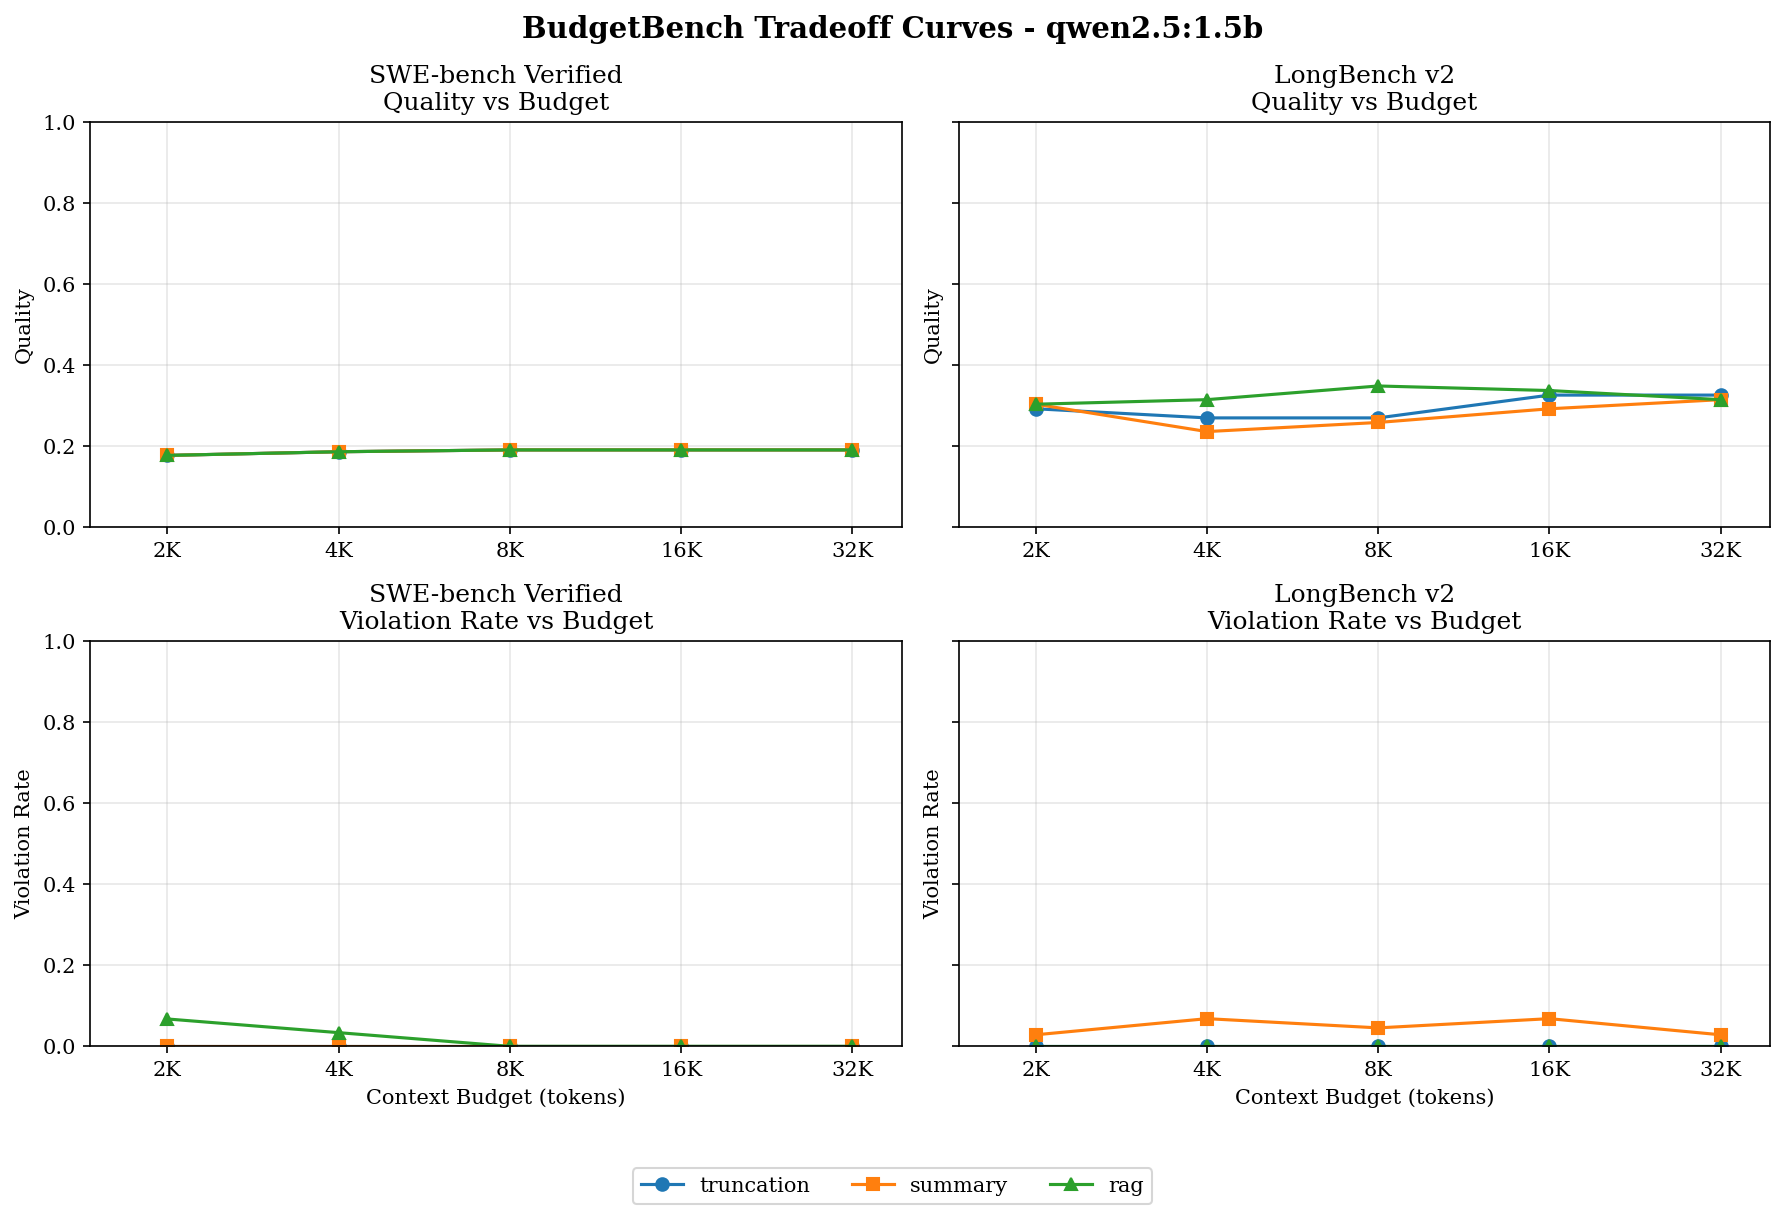
\includegraphics[width=\textwidth]{../results/figures/tradeoff_curves_qwen2_5_1_5b.png}
  \caption{Quality and budget-violation curves for the 89-item-per-task pilot run. Blue circles denote truncation, orange squares denote summary, and green triangles denote retrieval-augmented generation (RAG). SWE quality is the patch-similarity proxy; LongBench v2 quality is exact-match accuracy.}
  \label{fig:tradeoff_89item}
\end{figure}

\begin{figure}[t]
  \centering
  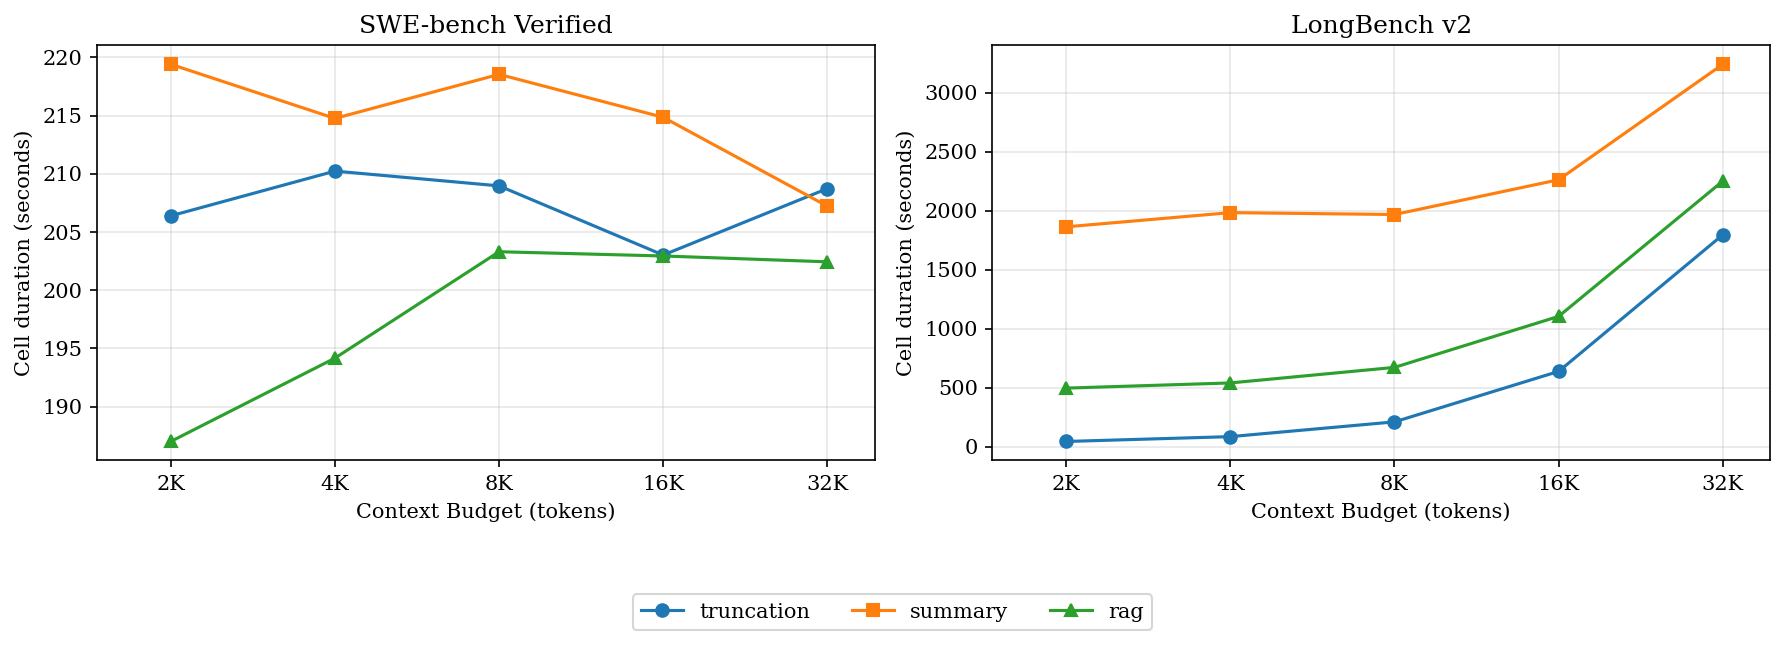
\includegraphics[width=\textwidth]{../results/figures/duration_curves_qwen2_5_1_5b.png}
  \caption{Cell-level runtime by task, strategy, and active context budget. Blue circles denote truncation, orange squares denote summary, and green triangles denote retrieval-augmented generation (RAG).}
  \label{fig:duration_89item}
\end{figure}

\begin{figure}[t]
  \centering
  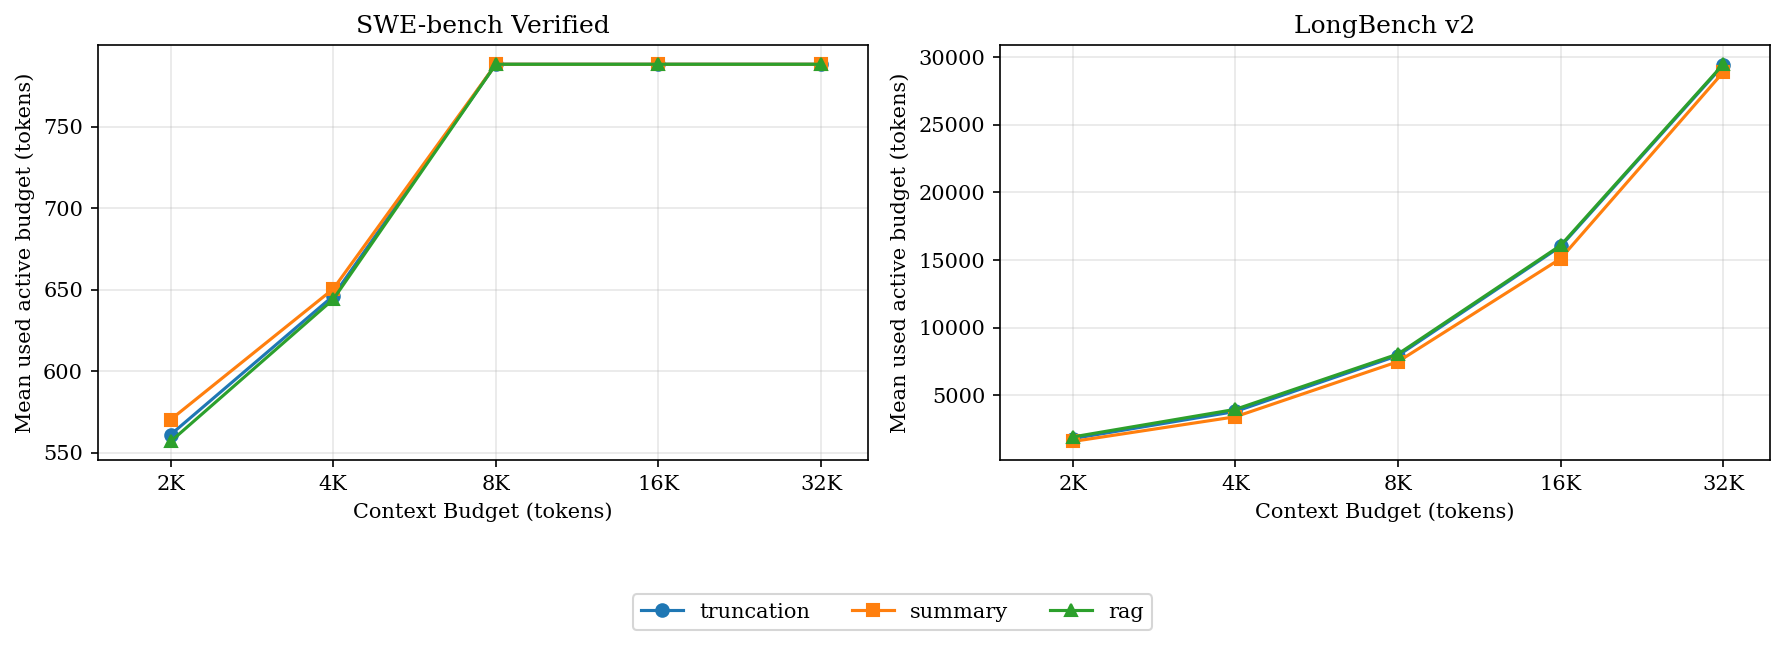
\includegraphics[width=\textwidth]{../results/figures/used_budget_curves_qwen2_5_1_5b.png}
  \caption{Mean used active budget by task, strategy, and tier. Blue circles denote truncation, orange squares denote summary, and green triangles denote retrieval-augmented generation (RAG).}
  \label{fig:used_budget_89item}
\end{figure}


\subsection{Supplementary Model and Multimodal Checks}

Table~\ref{tab:model_transfer_gemma4} reports the usable rows from the follow-up
small-model sweep.  This is not a ranking comparison with the 89-item run: it
uses only three LongBench v2 items and only the 2K--8K tiers.  Its purpose is
to verify that the \BudgetBench{} protocol can be reused across newly installed
Ollama tags and that result reporting can exclude uninformative runs for the
current text-only task.  On this slice, \texttt{gemma4:e2b} produced nonzero
exact-match accuracy in every reported cell.  RAG matched or exceeded
truncation while incurring roughly double the mean cell duration.

Table~\ref{tab:multimodal_probe} reports the separate native multimodal
probe.  The six generated items use simple image-plus-text prompts, so the
result should not be read as evidence about real-world visual reasoning.  The
probe verifies that the local serving stack can carry image payloads and that
\BudgetBench{} can record multimodal artifacts without mixing them into the
text-only LongBench budget table.

\begin{table}[t]
\centering
\caption{Nonzero rows from the additional small-model LongBench v2 transfer diagnostic.  Retrieval-augmented generation (RAG) denotes the episodic retrieval baseline.  The check used three LongBench v2 items, the 2K--8K budget tiers, temperature 0.0, and Ollama's OpenAI-compatible endpoint.  These local alias rows lack complete model provenance and are not benchmark claims.  Zero-accuracy and endpoint-mismatch rows from the same sweep are reported separately in Table~\ref{tab:model_transfer_excluded}.}
\label{tab:model_transfer_gemma4}
\begin{tabular}{llcccc}
\toprule
Model & Strategy & 2K & 4K & 8K & Mean duration (s) \\
\midrule
\texttt{gemma4:e2b} & Truncation & 0.33 & 0.67 & 0.67 & 23.7 \\
\texttt{gemma4:e2b} & RAG & 0.67 & 0.67 & 0.67 & 46.6 \\
\bottomrule
\end{tabular}
\end{table}

\begin{table}[t]
\centering
\caption{Zero-accuracy and endpoint-mismatch rows from the additional small-model LongBench v2 transfer diagnostic.  Retrieval-augmented generation (RAG) denotes the episodic retrieval baseline.  All entries use three LongBench v2 items and report exact-match accuracy at 2K, 4K, and 8K.  These local alias rows lack complete model provenance and are not benchmark claims.}
\label{tab:model_transfer_excluded}
\resizebox{\textwidth}{!}{%
\begin{tabular}{llcl}
\toprule
Model & Strategy & Accuracy at 2K / 4K / 8K & Reporting note \\
\midrule
\texttt{qwen3-vl:2b} & Truncation & 0.00 / 0.00 / 0.00 & Text-only endpoint check \\
\texttt{qwen3-vl:2b} & RAG & 0.00 / 0.00 / 0.00 & Text-only endpoint check \\
\texttt{qwen3.5:0.8b} & Truncation & 0.00 / 0.00 / 0.00 & Zero exact-match signal \\
\texttt{qwen3.5:0.8b} & RAG & 0.00 / 0.00 / 0.00 & Zero exact-match signal \\
\texttt{qwen3.5:2b} & Truncation & 0.00 / 0.00 / 0.00 & Zero exact-match signal; 1,024-token output cap \\
\texttt{qwen3.5:2b} & RAG & 0.00 / 0.00 / 0.00 & Zero exact-match signal; 1,024-token output cap \\
\bottomrule
\end{tabular}
}
\end{table}

\begin{table}[t]
\centering
\caption{Native multimodal probe result for a generated six-item image question answering (QA) set.  Each item contains a simple rendered colored shape and a multiple-choice text question.  This local alias row is a modality-path diagnostic, not a benchmark-scale vision evaluation or reproducible model claim.}
\label{tab:multimodal_probe}
\begin{tabular}{llccc}
\toprule
Model & Modality & Items & Accuracy & Mean duration (s) \\
\midrule
\texttt{qwen3-vl:2b} & Image + text & 6 & 1.00 & 1.7 \\
\bottomrule
\end{tabular}
\end{table}


\section{Discussion}

\subsection{Quality Curves Are Not Guaranteed to Be Monotonic}

The pilot reinforces a point that long-context evaluation has repeatedly
exposed: increasing the active context budget does not necessarily improve
quality.  A larger prompt can include more evidence, but it can also include
more distractors and can change the relative position of salient information.
For a small model, the additional content may be more harmful than helpful.
This is especially visible in LongBench-style tasks, where the model must
select a single answer from a long context rather than merely continue a short
conversation.

\subsection{Compliance Failures Are First-Class Results}

Budget violations are not peripheral errors.  They tell us whether a memory
strategy can actually operate at a requested tier.  In the pilot, tight budgets
can fail when the irreducible system-plus-query prompt already exceeds the
budget after strategy fallback.  Such failures should be counted separately
from low task quality: a strategy that fails to produce a budget-compliant
prompt is operationally different from one that produces a compliant but wrong
answer.

\subsection{Latency Can Dominate Strategy Choice}

The summary-buffer baseline is conceptually attractive because it attempts to
preserve global state rather than dropping it.  In practice, it can add a full
extra generation call before the answer call.  On long-context tasks, that
extra call dominates runtime.  A memory strategy that improves accuracy by a
small amount may still be unattractive if it multiplies latency.  Conversely,
a retrieval strategy can have a fixed embedding cost but avoid repeated
generation-based compression.  This is why \BudgetBench{} reports duration and
budget utilization alongside quality.

\subsection{Pilot Scope}

The current run is intentionally small.  It demonstrates the measurement
surface, not final superiority of one strategy over another.  A
benchmark-scale study should increase the item count, use stronger local
models, evaluate official SWE-bench resolution, include tau-bench state
grading, add multimodal task families before making claims about
vision-language memory, and report confidence intervals.  The pilot establishes
the path from local serving to budget-constrained logs, analysis, tables,
figures, and a reproducible paper artifact.

\section{Threats to Validity}

\paragraph{Internal validity.}
The runner uses a tokenizer function based on \texttt{tiktoken} rather than
the exact Ollama model tokenizer.  This is acceptable for a pilot but should be
replaced with model-specific token accounting in a final benchmark.  The
summary strategy uses the same small model for compression; a stronger
summarizer could change the results.  The RAG strategy uses generic embeddings
and simple message-level retrieval rather than task-optimized chunking.

\paragraph{External validity.}
The model is small, the sample contains 89 items per task, and only two task
families are included.  Larger local models may benefit more from larger
budgets.  Production agents may maintain cross-item or cross-session memory,
whereas this pilot resets strategy state between items.  The results should
therefore be interpreted as a validation of the protocol and implementation,
not as a general statement about all local memory strategies.  The additional
\texttt{gemma4:e2b} sweep is even narrower: it is a three-item transfer check
and should be read only as evidence that the protocol transfers to another
local tag under controlled reporting rules.

\paragraph{Construct validity.}
The SWE patch-similarity proxy measures overlap with the reference patch, not
actual repository repair.  It can reward patches that touch the right file or
line without being executable fixes.  LongBench v2 exact-match scoring is more
direct, but 89 questions are still too few for definitive estimates.  Future
studies should use official task graders and report uncertainty.

\paragraph{Multimodal validity.}
The primary benchmark run does not contain image, video, chart, or
document-page inputs.  The added image QA probe verifies the native
image-plus-text path on generated colored shapes, but it is too small and too
simple to support claims about real multimodal memory.  Therefore, this paper
should be read as adding a multimodal data path and extension plan, not as
claiming benchmark-scale multimodal performance.

\section{Planned Extensions}

The next version of \BudgetBench{} should expand in five directions.  First,
it should replace proxy SWE grading with official containerized evaluation.
Second, it should include tau-bench or tau2-bench once the local data
dependency is installed, because tool-use chains stress memory in ways that
single-call QA does not.  Third, it should add richer strategy families:
LLMLingua-2 compression, Mem0, Letta/MemGPT-style hierarchical memory, and
hybrid retrieval-summary policies.  Fourth, it should add repeated trials and
confidence intervals so strategy crossovers can be distinguished from sampling
noise.  Fifth, it should add multimodal tasks with native visual inputs and
multimodal memory policies.  Examples include document-page QA where the active
budget controls OCR text plus image references, chart QA where retrieval
chooses both visual crops and textual evidence, and tool-agent tasks where
screenshots or UI state are part of the memory trace.

\section{Conclusion}

\BudgetBench{} operationalizes an under-standardized evaluation
question: how do memory strategies trade quality, budget compliance, and
latency when active context is fixed?  The expanded 89-item pilot run
demonstrates that this question can be evaluated locally with a small model,
deterministic graders, five budget tiers, and swappable strategy baselines.
This paper provides the protocol, literature positioning, result tables,
operational metrics, and reproducibility record needed to inspect the pilot.
The strongest claim is methodological rather than rank-oriented:
fixed-budget evaluation reveals failure modes that standard long-context
evaluation can hide, and those failure modes are central to practical local
agent deployment.

\clearpage
\appendix

\section{Reproducibility Checklist}

\begin{longtable}{p{0.28\textwidth}p{0.62\textwidth}}
\caption{Pilot reproducibility checklist.}\\
\toprule
Item & Value \\
\midrule
\endfirsthead
\toprule
Item & Value \\
\midrule
\endhead
Run date & June 16, 2026 \\
Model & \RunModel{} served through Ollama \\
Endpoint & \OllamaEndpoint{} \\
Run identifier & \RunId{} \\
Budget tiers & 2,048; 4,096; 8,192; 16,384; 32,768 active input tokens \\
Tasks & SWE-bench Verified scaffold; LongBench v2 multiple-choice QA \\
Strategies & Truncation, summary buffer, episodic RAG \\
Items per task & 89 \\
Temperature & 0.0 \\
Maximum generated tokens & 512 \\
Random seed & 42 \\
Primary raw logs & \path{logs/full_study/final_qwen25_15b_89items/summary.jsonl} \\
Primary aggregate CSV & \path{results/full_study_qwen2_5_1_5b_89items.csv} \\
Additional filtered model sweep & \path{results/model_compare_small_long3.csv}; reported rows limited to \texttt{gemma4:e2b} because zero-accuracy or endpoint-anomalous rows are excluded from paper tables \\
Native multimodal probe artifacts & \path{results/multimodal_smoke_qwen3_vl_2b.csv}; generated PNGs in \path{results/multimodal_smoke/} \\
\bottomrule
\end{longtable}

\section{Task Specifications}

\subsection{SWE-Bench Verified Scaffold}

\begin{longtable}{p{0.24\textwidth}p{0.66\textwidth}}
\caption{SWE scaffold task card.}\\
\toprule
Field & Description \\
\midrule
\endfirsthead
\toprule
Field & Description \\
\midrule
\endhead
Purpose & Evaluate whether a local model can transform a natural-language bug report and hints into a patch-like diff under constrained context. \\
Input format & System prompt instructing the model to produce only a unified diff; user prompt containing the problem statement and available hints. \\
Prediction format & Text response from which the first \texttt{diff --git} block is extracted. \\
Grader & Deterministic patch-similarity proxy using file recall and changed-line overlap. \\
Strength & Low-cost, deterministic, and fast enough for repeated budget sweeps. \\
Limitation & Does not execute tests; cannot be interpreted as official SWE-bench resolution. \\
Scaling path & Replace proxy with official SWE-bench containerized oracle; stratify by repository, patch size, and issue type. \\
\bottomrule
\end{longtable}

\subsection{LongBench v2}

\begin{longtable}{p{0.24\textwidth}p{0.66\textwidth}}
\caption{LongBench v2 task card.}\\
\toprule
Field & Description \\
\midrule
\endfirsthead
\toprule
Field & Description \\
\midrule
\endhead
Purpose & Evaluate long-context evidence selection and answer-choice discrimination under fixed active budgets. \\
Input format & System prompt, context chunks, question, and four answer choices. \\
Prediction format & One of A, B, C, or D, extracted from the model response. \\
Grader & Exact-match letter comparison. \\
Strength & Deterministic and directly compatible with budgeted prompt manipulation. \\
Limitation & Small pilot subset; exact-match increments are coarse at low sample counts. \\
Scaling path & Increase sample count; stratify by context length, evidence dispersion, and reasoning type. \\
\bottomrule
\end{longtable}

\section{Strategy Specifications}

\subsection{Truncation}

Truncation is the simplest baseline.  It preserves the system prompt and then
walks backward through the message list, retaining the newest messages that fit
inside the remaining budget.  Its primary failure mode is the loss of older
evidence, including evidence that may be decisive.  Its advantage is that it
requires no extra model calls, no embedding model, and no external memory
store.  In a budget benchmark, truncation is the minimal memory-management
baseline that more complex strategies should be compared against.

\subsection{Summary Buffer}

The summary-buffer strategy attempts to compress evicted context into a
shorter natural-language state.  The pilot implementation reserves a portion
of the budget for a summary, chooses recent messages to retain, and asks the
local model to summarize the evicted messages.  This baseline can preserve
global state, but it introduces additional generation cost and can suffer from
summary drift.  In the pilot, summary is especially expensive on LongBench
because long contexts trigger repeated compression calls.

\subsection{Episodic RAG}

The RAG baseline indexes intermediate messages and retrieves chunks relevant
to the current query.  It is a direct adaptation of retrieval-augmented
generation to the prompt-budget setting \citep{lewis2020rag}.  Its advantage
is selectivity: it can recover older evidence without including the full
history.  Its limitations are query dependence, chunking sensitivity, embedding
cost, and the possibility that relevant information is not semantically close
to the final question.

\section{Metric Definitions}

\subsection{Quality}

Quality is task-specific.  For LongBench v2 it is exact-match accuracy:
\[
  \mathrm{Acc} = \frac{1}{N}\sum_i \mathbb{1}[\hat{a}_i = a_i].
\]
For the SWE scaffold it is a continuous patch-similarity score:
\[
  \mathrm{SWEProxy} = 0.4 \cdot \mathrm{FileRecall} + 0.6 \cdot \mathrm{LineOverlap}.
\]
The proxy is useful for pilot measurement but should be replaced by official
test execution for benchmark claims.

\subsection{Violation Rate}

Violation rate is the mean retry-level budget failure rate over items in a
cell.  If a strategy returns a prompt exceeding the active tier, the runner
logs the violation and retries.  A cell can therefore have nonzero quality and
nonzero violations if some items succeed while others fail under the tier.

\subsection{Utilization and Peak Budget}

Mean used budget measures how many prompt tokens the strategy actually sends
on successful calls.  Maximum peak budget records the largest token count
observed during enforcement, including failed attempts.  These metrics separate
conservative strategies that under-use budget from strategies that operate
near the ceiling.

\subsection{Duration}

Duration is wall-clock time for the cell.  It includes strategy overhead,
embedding or summarization calls, final model calls, and dataset-item loop
overhead.  Duration is machine-dependent, but it remains operationally useful
because the benchmark is explicitly about local deployment regimes.

\section{Full Operational Tables}

\begin{table}[p]
\centering
\caption{Full quality matrix for the 89-item-per-task run. Retrieval-augmented generation (RAG) denotes the episodic retrieval baseline. LongBench v2 values are exact-match accuracy. SWE values are patch-similarity proxy scores and are not official SWE-bench accuracy.}
\label{tab:app_quality}
\begin{tabular}{llccccc}
\toprule
Task & Strategy & 2K & 4K & 8K & 16K & 32K \\
\midrule
\multirow{3}{*}{SWE} & Truncation & 0.18 & 0.19 & 0.19 & 0.19 & 0.19 \\
& Summary & 0.18 & 0.19 & 0.19 & 0.19 & 0.19 \\
& RAG & 0.18 & 0.19 & 0.19 & 0.19 & 0.19 \\
\midrule
\multirow{3}{*}{LongBench v2} & Truncation & 0.29 & 0.27 & 0.27 & 0.33 & 0.33 \\
& Summary & 0.30 & 0.24 & 0.26 & 0.29 & 0.31 \\
& RAG & 0.30 & 0.31 & 0.35 & 0.34 & 0.31 \\
\bottomrule
\end{tabular}
\end{table}

\begin{table}[p]
\centering
\caption{Full budget-violation matrix for the 89-item-per-task run. Retrieval-augmented generation (RAG) denotes the episodic retrieval baseline.}
\label{tab:app_violation}
\begin{tabular}{llccccc}
\toprule
Task & Strategy & 2K & 4K & 8K & 16K & 32K \\
\midrule
\multirow{3}{*}{SWE} & Truncation & 0.00 & 0.00 & 0.00 & 0.00 & 0.00 \\
& Summary & 0.00 & 0.00 & 0.00 & 0.00 & 0.00 \\
& RAG & 0.07 & 0.03 & 0.00 & 0.00 & 0.00 \\
\midrule
\multirow{3}{*}{LongBench v2} & Truncation & 0.00 & 0.00 & 0.00 & 0.00 & 0.00 \\
& Summary & 0.03 & 0.07 & 0.05 & 0.07 & 0.03 \\
& RAG & 0.00 & 0.00 & 0.00 & 0.00 & 0.00 \\
\bottomrule
\end{tabular}
\end{table}

\begin{table}[p]
\centering
\caption{Mean used active budget in tokens. Retrieval-augmented generation (RAG) denotes the episodic retrieval baseline.}
\label{tab:app_mean_used}
\begin{tabular}{llccccc}
\toprule
Task & Strategy & 2K & 4K & 8K & 16K & 32K \\
\midrule
\multirow{3}{*}{SWE} & Truncation & 561 & 646 & 788 & 788 & 788 \\
& Summary & 570 & 650 & 788 & 788 & 788 \\
& RAG & 557 & 644 & 788 & 788 & 788 \\
\midrule
\multirow{3}{*}{LongBench v2} & Truncation & 1,797 & 3,803 & 7,937 & 16,012 & 29,411 \\
& Summary & 1,584 & 3,412 & 7,489 & 15,111 & 28,899 \\
& RAG & 1,919 & 3,961 & 8,052 & 16,088 & 29,483 \\
\bottomrule
\end{tabular}
\end{table}

\begin{table}[p]
\centering
\caption{Maximum observed peak budget in tokens. Retrieval-augmented generation (RAG) denotes the episodic retrieval baseline.}
\label{tab:app_peak}
\begin{tabular}{llccccc}
\toprule
Task & Strategy & 2K & 4K & 8K & 16K & 32K \\
\midrule
\multirow{3}{*}{SWE} & Truncation & 1,973 & 3,299 & 4,542 & 4,542 & 4,542 \\
& Summary & 1,973 & 3,299 & 4,542 & 4,542 & 4,542 \\
& RAG & 4,542 & 4,542 & 4,542 & 4,542 & 4,542 \\
\midrule
\multirow{3}{*}{LongBench v2} & Truncation & 2,028 & 4,092 & 8,180 & 16,382 & 32,762 \\
& Summary & 2,153 & 4,398 & 8,439 & 16,658 & 33,011 \\
& RAG & 2,048 & 4,094 & 8,192 & 16,384 & 32,768 \\
\bottomrule
\end{tabular}
\end{table}

\begin{table}[p]
\centering
\caption{Cell duration in seconds. Retrieval-augmented generation (RAG) denotes the episodic retrieval baseline.}
\label{tab:app_duration}
\begin{tabular}{llccccc}
\toprule
Task & Strategy & 2K & 4K & 8K & 16K & 32K \\
\midrule
\multirow{3}{*}{SWE} & Truncation & 206.4 & 210.2 & 209.0 & 203.0 & 208.7 \\
& Summary & 219.4 & 214.8 & 218.5 & 214.9 & 207.2 \\
& RAG & 187.0 & 194.2 & 203.3 & 202.9 & 202.4 \\
\midrule
\multirow{3}{*}{LongBench v2} & Truncation & 43.3 & 84.3 & 209.4 & 637.2 & 1794.8 \\
& Summary & 1862.3 & 1982.7 & 1966.8 & 2261.3 & 3240.0 \\
& RAG & 495.5 & 539.3 & 671.1 & 1103.5 & 2250.0 \\
\bottomrule
\end{tabular}
\end{table}

\begin{longtable}{lllrrrrr}
\caption{Flat per-cell aggregate data for audit.}\\
\toprule
Model & Task & Strategy & Budget & Quality & Viol. & Mean Used & Duration (s) \\
\midrule
\endfirsthead
\toprule
Model & Task & Strategy & Budget & Quality & Viol. & Mean Used & Duration (s) \\
\midrule
\endhead
qwen2.5:1.5b & long & rag & 2,048 & 0.303 & 0.000 & 1919.2 & 495.5 \\
qwen2.5:1.5b & long & rag & 4,096 & 0.315 & 0.000 & 3960.8 & 539.3 \\
qwen2.5:1.5b & long & rag & 8,192 & 0.348 & 0.000 & 8052.4 & 671.1 \\
qwen2.5:1.5b & long & rag & 16,384 & 0.337 & 0.000 & 16087.7 & 1103.5 \\
qwen2.5:1.5b & long & rag & 32,768 & 0.315 & 0.000 & 29482.7 & 2250.0 \\
qwen2.5:1.5b & long & summary & 2,048 & 0.303 & 0.028 & 1584.4 & 1862.3 \\
qwen2.5:1.5b & long & summary & 4,096 & 0.236 & 0.068 & 3412.5 & 1982.7 \\
qwen2.5:1.5b & long & summary & 8,192 & 0.258 & 0.045 & 7488.5 & 1966.8 \\
qwen2.5:1.5b & long & summary & 16,384 & 0.292 & 0.068 & 15110.9 & 2261.3 \\
qwen2.5:1.5b & long & summary & 32,768 & 0.315 & 0.028 & 28898.8 & 3240.0 \\
qwen2.5:1.5b & long & truncation & 2,048 & 0.292 & 0.000 & 1796.6 & 43.3 \\
qwen2.5:1.5b & long & truncation & 4,096 & 0.270 & 0.000 & 3803.2 & 84.3 \\
qwen2.5:1.5b & long & truncation & 8,192 & 0.270 & 0.000 & 7936.5 & 209.4 \\
qwen2.5:1.5b & long & truncation & 16,384 & 0.326 & 0.000 & 16011.7 & 637.2 \\
qwen2.5:1.5b & long & truncation & 32,768 & 0.326 & 0.000 & 29410.9 & 1794.8 \\
qwen2.5:1.5b & swe & rag & 2,048 & 0.177 & 0.067 & 556.8 & 187.0 \\
qwen2.5:1.5b & swe & rag & 4,096 & 0.186 & 0.034 & 644.1 & 194.2 \\
qwen2.5:1.5b & swe & rag & 8,192 & 0.191 & 0.000 & 788.3 & 203.3 \\
qwen2.5:1.5b & swe & rag & 16,384 & 0.191 & 0.000 & 788.3 & 202.9 \\
qwen2.5:1.5b & swe & rag & 32,768 & 0.191 & 0.000 & 788.3 & 202.4 \\
qwen2.5:1.5b & swe & summary & 2,048 & 0.177 & 0.000 & 570.2 & 219.4 \\
qwen2.5:1.5b & swe & summary & 4,096 & 0.186 & 0.000 & 650.5 & 214.8 \\
qwen2.5:1.5b & swe & summary & 8,192 & 0.191 & 0.000 & 788.3 & 218.5 \\
qwen2.5:1.5b & swe & summary & 16,384 & 0.191 & 0.000 & 788.3 & 214.9 \\
qwen2.5:1.5b & swe & summary & 32,768 & 0.191 & 0.000 & 788.3 & 207.2 \\
qwen2.5:1.5b & swe & truncation & 2,048 & 0.177 & 0.000 & 561.0 & 206.4 \\
qwen2.5:1.5b & swe & truncation & 4,096 & 0.186 & 0.000 & 646.2 & 210.2 \\
qwen2.5:1.5b & swe & truncation & 8,192 & 0.191 & 0.000 & 788.3 & 209.0 \\
qwen2.5:1.5b & swe & truncation & 16,384 & 0.191 & 0.000 & 788.3 & 203.0 \\
qwen2.5:1.5b & swe & truncation & 32,768 & 0.191 & 0.000 & 788.3 & 208.7 \\
\bottomrule
\end{longtable}

\begin{figure}[p]
  \centering
  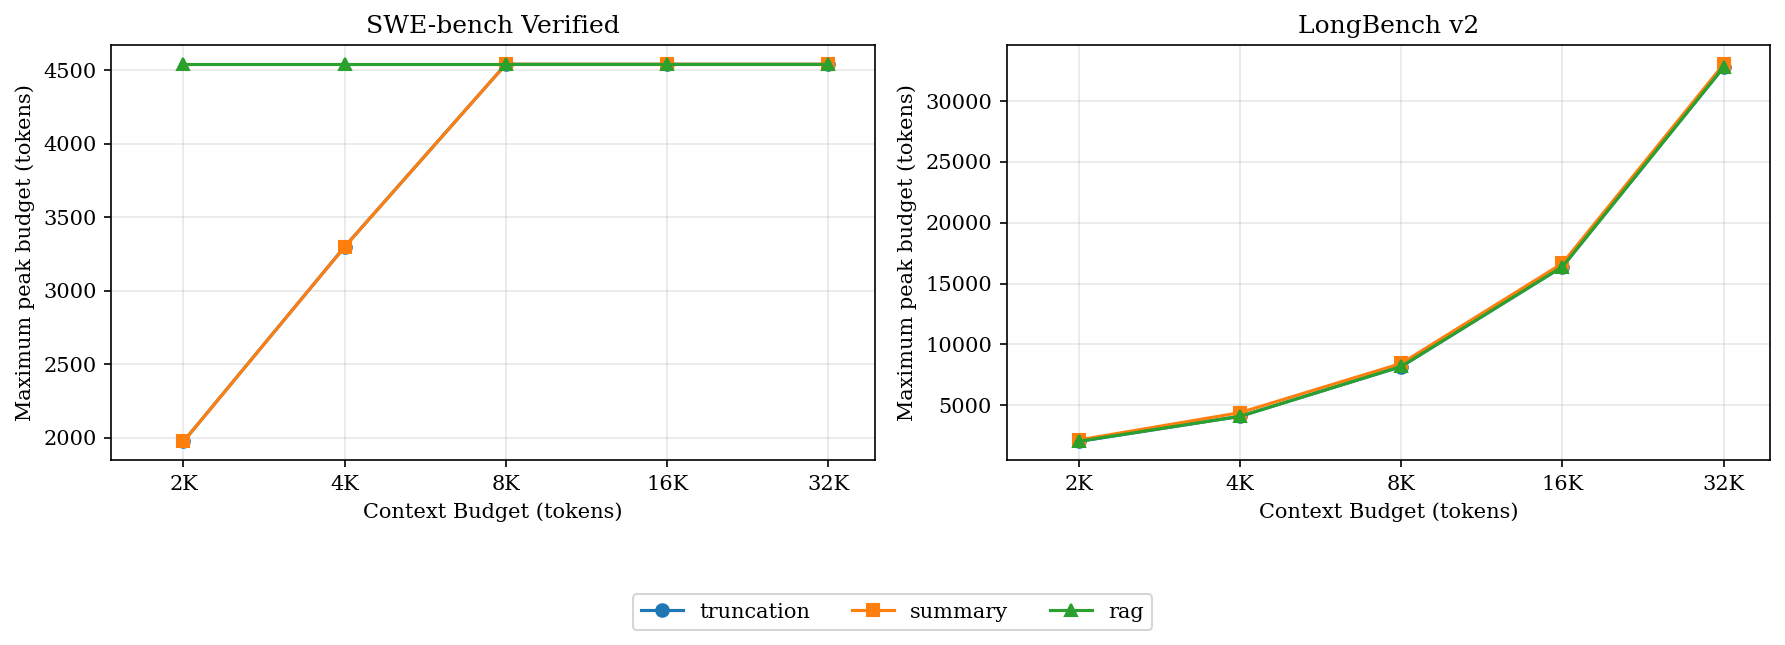
\includegraphics[width=\textwidth]{../results/figures/peak_budget_curves_qwen2_5_1_5b.png}
  \caption{Maximum peak budget observed in each cell. Blue circles denote truncation, orange squares denote summary, and green triangles denote retrieval-augmented generation (RAG).}
  \label{fig:peak_budget_89item}
\end{figure}


\section{Artifact and Reporting Policy}

\subsection{Artifact Boundaries}

The artifact is a benchmark scaffold, not a static dataset release.  The code
defines a protocol and adapters for existing datasets.  The logs generated by
the pilot are reproducibility artifacts for this paper.  Future benchmark
submissions should preserve raw logs, model hashes, dependency versions, and
hardware metadata so that budget-compliance failures can be audited.

\subsection{Submission Policy}

A public \BudgetBench{} benchmark should require strategy implementations to
declare all external dependencies, whether they call additional LLMs, whether
they use persistent state across items, and whether they require remote APIs.
Strategies that use remote proprietary services should be reported separately
from local-only strategies because they change the deployment regime being
measured.

\subsection{Recommended Reporting Template}

Every benchmark report should include: model name and quantization, serving
stack, tokenizer used for enforcement, budget tiers, task subset, number of
items, random seed, decoding parameters, strategy names, quality curves,
violation curves, mean used budget, peak budget, latency, and raw log location.
Without these fields, it is difficult to distinguish a genuine memory-strategy
effect from a serving or measurement artifact.

\section{Additional Limitations}

This paper makes several conservative claims.  First, it does not claim
novelty on long-context evaluation alone; RULER, HELMET, LongBench,
and LongBench v2 already address long-context measurement from different
angles \citep{bai2023longbench,bai2024longbenchv2,hsieh2024ruler,yen2024helmet}.
Second, it does not claim that retrieval, summary, or truncation is globally
best.  The pilot sample is too small.  Third, it does not claim official
SWE-bench results.  The SWE column is clearly labeled as a scaffold proxy.
The novelty is the conjunction of fixed active budget, swappable memory
strategy, local model serving, deterministic logging, and task-level quality
measurement.

\section{Statistical Scaling Plan}

The pilot tables in this paper are intentionally small, but the benchmark
protocol is designed to scale to statistically meaningful comparisons.  This
appendix section specifies how a larger \BudgetBench{} study should move from
artifact validation to inference.  The most important principle is that every
claim about strategy dominance must be tied to a task, model, budget tier, and
uncertainty estimate.  Statements such as ``RAG is best'' are underspecified.
The benchmark should instead support statements such as ``for model $M$ on
LongBench v2 items with contexts in the 8K--32K range, RAG has higher mean
exact-match accuracy than truncation at the 2K active budget with a bootstrap
95\% confidence interval that excludes zero.''

\subsection{Recommended Estimands}

For a fixed model $M$, task family $T$, strategy $s$, and budget $B$, the
primary estimand is expected task quality $Q(s,B,T,M)$.  The most useful
comparative estimand is the paired difference between two strategies on the
same items:
\[
  \Delta(s_a,s_b,B,T,M) =
  \frac{1}{N}\sum_{i=1}^{N}
  \left[g(M(s_a(H_i,B)),x_i) - g(M(s_b(H_i,B)),x_i)\right].
\]
Pairing is important because task difficulty can dominate strategy effects.
The same item may be easy for every strategy or impossible for every strategy.
A paired estimate removes much of that item-level variance and focuses the
comparison on whether the strategy changed the outcome.

For latency, the analogous estimand is the paired runtime difference or ratio.
Ratios are often easier to interpret operationally.  For example, if summary
buffer achieves the same quality as truncation but costs $10\times$ more
wall-clock time at 32K, then the strategy is unlikely to be attractive for an
interactive local agent.  For budget compliance, the estimand is the failure
probability at a tier.  A strategy with high quality conditional on success
but frequent budget failure should not be ranked as reliable.

\subsection{Confidence Intervals}

For exact-match tasks, a binomial interval is a useful first diagnostic, but
paired bootstrap intervals are preferable when comparing strategies.  For
continuous proxy scores such as the current SWE patch-similarity metric,
non-parametric bootstrap over items is appropriate.  A full study should report
the interval around each strategy's quality curve and the interval around each
pairwise difference curve.  The pilot does not report such intervals because a
single 89-item run is still an artifact-validation study rather than a powered
benchmark comparison; presenting tight intervals from this run would create
false precision.

\subsection{Sample Size Guidance}

The required sample size depends on the effect size that the benchmark is
expected to detect.  Exact-match tasks with four-way multiple-choice answers
have high variance at small $N$.  With $N=9$, one item changes accuracy by
0.111.  With $N=50$, one item changes accuracy by 0.02.  With the present
$N=89$ pilot, one item changes accuracy by approximately 0.0112.  With
$N=100$, one item changes accuracy by 0.01.  For pilot validation, this
89-item run is enough to exercise the full matrix and reduce coarse rounding
artifacts.  For a paper-quality strategy comparison, $N=100$ or more per task
family should be used when claiming budget crossovers.

\begin{longtable}{p{0.18\textwidth}p{0.24\textwidth}p{0.44\textwidth}}
\caption{Recommended study sizes by claim type.}\\
\toprule
Study type & Suggested items & Appropriate claims \\
\midrule
\endfirsthead
\toprule
Study type & Suggested items & Appropriate claims \\
\midrule
\endhead
Smoke test & 1--3 per task & Dependency wiring, API reachability, log creation, and gross runtime estimates. \\
Pilot & 5--15 per task & End-to-end protocol validation, visible failure modes, qualitative curve shapes, and paper artifact generation. \\
Focused ablation & 30--50 per task & Coarse strategy comparisons within one task family and one model, with wide uncertainty intervals. \\
Benchmark paper & 100+ per task family & Strategy ranking at named budget tiers, paired difference estimates, and task-stratified analysis. \\
Leaderboard & Full public subset or fixed hidden split & Submission ranking, regression testing, and longitudinal tracking of strategy improvements. \\
\bottomrule
\end{longtable}

\subsection{Stratification}

Random sampling is not enough for a benchmark paper.  SWE-bench items should be
stratified by repository, patch size, issue text length, and whether the fix is
localized or cross-file.  LongBench v2 items should be stratified by context
length, evidence dispersion, and reasoning type.  Tau-bench items should be
stratified by tool-call count, policy-document length, and whether the task
requires state mutation.  Stratification prevents a small number of easy or
pathological items from dominating a curve.

\section{Failure Taxonomy}

Budget-tiered evaluation creates failure modes that do not appear in standard
single-prompt evaluation.  The table below gives a taxonomy that should be used
when annotating future \BudgetBench{} runs.  The pilot already exhibits several
of these cases: RAG can violate tight SWE budgets when the irreducible prompt
is too large, summary can violate LongBench budgets after compression, and
LongBench quality can decrease as budget increases.

\begin{longtable}{p{0.18\textwidth}p{0.25\textwidth}p{0.43\textwidth}}
\caption{Failure taxonomy for budget-tiered memory evaluation.}\\
\toprule
Failure type & Observable symptom & Interpretation and remediation \\
\midrule
\endfirsthead
\toprule
Failure type & Observable symptom & Interpretation and remediation \\
\midrule
\endhead
Irreducible prompt overflow & System prompt plus final query exceeds the active budget. & The task formatter itself must be shortened, or the tier should be marked infeasible for that task. Strategy changes cannot fix a prompt whose fixed component is already too large. \\
Strategy overflow & Processed messages exceed budget after strategy application. & The strategy needs stricter accounting, smaller reserves, or token-aware chunking. This is a compliance bug or design mismatch. \\
Compression drift & Summary strategy is compliant but loses decisive evidence. & Evaluate summary faithfulness, add extraction constraints, or use retrieval-backed summaries. \\
Retrieval miss & RAG is compliant but selects irrelevant chunks. & Improve chunk granularity, query formulation, embedding model, or hybrid recency/relevance scoring. \\
Distractor overload & Larger budgets reduce exact-match accuracy. & More context is not always better; inspect evidence position and distractor density. Consider reranking or evidence-focused compression. \\
Latency explosion & Quality is stable but duration grows sharply. & Strategy may be operationally dominated despite quality. Report latency alongside accuracy. \\
Metric mismatch & Proxy quality improves but official task success does not. & Replace proxy with official grader before making benchmark claims. This is especially important for SWE. \\
State leakage & Cross-item memory improves later items unexpectedly. & Reset strategy state or explicitly evaluate persistent-memory regimes separately. \\
Serving artifact & Model output format changes due to endpoint behavior. & Pin serving stack, model tag, decoding parameters, and response extraction logic. \\
\bottomrule
\end{longtable}

\subsection{Interpreting Non-Monotonic Curves}

Non-monotonicity should not be automatically treated as noise.  In a
budgeted-memory setting, non-monotonic curves can be meaningful.  At small
budgets, a strategy may aggressively select only the most relevant evidence.
At larger budgets, it may include additional distractors that dilute attention
or alter the model's generation trajectory.  The LongBench RAG curve in the
89-item pilot is an example: the 8K budget has the highest RAG score.  The
proper next step is not to declare that smaller budgets are generally better,
but to inspect which items flip as context grows and whether those flips
correlate with evidence position, answer-choice similarity, or retrieved chunk
rank.

\subsection{Interpreting Equal SWE Scores}

The SWE proxy scores are equal across strategies at each tier in the pilot.
This does not imply that memory strategies are irrelevant for software
engineering tasks.  It more likely reflects three constraints: the sample is
small, the model is weak for patch generation, and the prompt for each item is
not yet a long-horizon agent trace.  A full SWE-oriented \BudgetBench{} study
should use an agent harness with repository browsing, tool outputs, and
multi-turn histories.  In that regime, strategy choice should matter more
because the context contains competing artifacts: issue text, retrieved files,
test failures, prior edits, and tool outputs.

\section{Scaling to a Full Benchmark Study}

This section outlines the expansion path from pilot artifact to larger
benchmark study.

\subsection{Phase 1: Measurement Hardening}

The first phase should replace approximate token counting with model-specific
token accounting wherever possible.  The runner should record dependency
versions, model hashes, hardware metadata, and serving parameters.  The metric
schema should be frozen so future analysis scripts do not need to infer which
log format was used.  The current analyzer fix is a small example of why this
matters: older logs used boolean violation fields, while current logs record
numeric retry-level violation rates.

\subsection{Phase 2: Task Expansion}

The second phase should wire official SWE-bench grading and tau-bench
state-comparison grading.  SWE should be run on a stratified subset first,
because official container execution is substantially more expensive than the
proxy grader.  Tau-bench should be pinned with a deterministic simulator
configuration.  LongBench v2 should be expanded to at least 50 items and
stratified by context length.

\subsection{Phase 3: Strategy Expansion}

The third phase should add LLMLingua-2, Mem0, Letta/MemGPT, and at least one
hybrid retrieval-summary strategy.  Each strategy should declare whether it is
local-only, whether it invokes an auxiliary model, and whether it maintains
persistent state.  These declarations should appear in result tables because
they affect deployment cost and reproducibility.

\subsection{Phase 4: Reporting and Release}

The fourth phase should publish raw logs, analysis scripts, figures, and a
frozen task subset.  A public evaluation service should accept strategy
submissions through the same \texttt{MemoryStrategy} interface and run them
against a hidden or versioned split.  The report should emphasize Pareto
frontiers rather than single scalar rankings: a strategy can be best at 2K and
dominated at 32K, or accurate but too slow for interactive use.

\begin{longtable}{p{0.16\textwidth}p{0.30\textwidth}p{0.38\textwidth}}
\caption{Expansion plan from pilot artifact to benchmark study.}\\
\toprule
Phase & Engineering work & Scientific output \\
\midrule
\endfirsthead
\toprule
Phase & Engineering work & Scientific output \\
\midrule
\endhead
Hardening & Tokenizer alignment, metadata capture, stable schemas, official dependency lock. & Auditable measurements and reproducible run manifests. \\
Task expansion & Official SWE grading, tau-bench data setup, larger LongBench v2 subsets. & Broader task coverage and deterministic multi-domain results. \\
Strategy expansion & LLMLingua-2, Mem0, Letta/MemGPT, hybrid policies, dependency declarations. & Strategy-family comparisons and local-vs-auxiliary cost analysis. \\
Statistical analysis & Paired bootstrap intervals, stratified estimates, repeated trials. & Defensible dominance and crossover claims. \\
Release & Public logs, fixed subsets, evaluation runner, submission documentation. & Community benchmark artifact suitable for datasets-and-benchmarks review. \\
\bottomrule
\end{longtable}

\section{Practitioner Guidance}

Developers applying \BudgetBench{} to their own agents should start with a
small connectivity check but should avoid over-interpreting it.  A one-item or
three-item run is useful for verifying that the model endpoint, task adapter,
and strategy dependencies work.  It is not useful for ranking strategies.  Once
the run is healthy, developers should choose a target deployment tier, such as
4K or 8K, and compare strategies there before paying for the full five-tier
sweep.  If the target tier exhibits high violation rates, strategy design
should focus on budget accounting before quality optimization.

Users should also inspect raw prompts.  Budget utilization numbers can reveal
that a strategy is conservative, but they cannot explain whether the retained
content is useful.  For retrieval strategies, users should inspect retrieved
chunks.  For summaries, users should inspect whether the summary preserved
decisive entities, constraints, and temporal ordering.  For truncation, users
should inspect what falls out of context.  The benchmark provides quantitative
signals; qualitative inspection remains essential for debugging.

Finally, larger budgets should not be assumed to be preferable.  If a smaller
budget performs better, the result may indicate that the strategy is filtering
distractors effectively.  The appropriate response is to analyze item-level
flips, not to discard the result because it violates a monotonicity expectation.

\section{Command Transcript Summary}

The main run command was:
\begin{verbatim}
python scripts/run_pilot.py \
  --full-study \
  --run-id final_qwen25_15b_89items \
  --model qwen2.5:1.5b \
  --tasks swe long \
  --strategies truncation summary rag \
  --limit-tasks 89
\end{verbatim}

The aggregate-analysis command was:
\begin{verbatim}
python scripts/analyze_results.py \
  --log-dirs logs/full_study/final_qwen25_15b_89items \
  --model qwen2.5:1.5b
\end{verbatim}

The figure-generation command was:
\begin{verbatim}
python scripts/plot_tradeoffs.py \
  --csv results/full_study_qwen2_5_1_5b_89items.csv \
  --model qwen2.5:1.5b
\end{verbatim}

\bibliography{references}
\bibliographystyle{plainnat}

\end{document}
